\documentclass[letterpaper,12pt]{article}
\usepackage[utf8]{inputenc}
\usepackage{enumitem}
\usepackage{hyperref}
\usepackage{graphicx}
\usepackage{textcomp}

\hypersetup{
  colorlinks=true,
  linkcolor=blue
}

\setenumerate{parsep=0em, listparindent=\parindent}

\title{Documentation for the nurses web tool}
\author{Benjamin Noland}
\date{}

\begin{document}

\maketitle
\tableofcontents

\section{Introduction}

This web tool allows you to explore trends in union membership and
union contract coverage for registered nurses in the United
States. You can use the tool to generate trend plots and chloropleth
maps showing how these quantities change over time, filtered and/or
grouped according to a variety of demographics (detailed below). The
tool uses data derived from the Current Population Survey (CPS) public
use microdata. For background information on the CPS, see the official
CPS website\footnote{\url{https://www.census.gov/programs-surveys/cps.html}}.

\section{Details of the data}

The tool operates on data derived from the Current Population Survey
(CPS) public use microdata (see the official CPS website for
information on the raw CPS data).  Each entry in the data used by the
tool corresponds to an individual interviewed as part of the CPS, and
includes various demographic data on that individual, as well as flags
indicating whether the individual is a union member or covered by a
union contract. Each entry also includes the year in which the
individual was interviewed, and a statistical weight used to calculate
union membership and union contract coverage proportions.

The following are descriptions of the variables in the data used by
the tool, including the possible values or levels that a particular
variable can assume:
\begin{description}[style=multiline,leftmargin=3cm,font=\normalfont]
\item[\texttt{year}] The year the individual was interviewed.

\item[\texttt{sex}] The individual's sex. This is derived from the CPS
  variable \texttt{PESEX}.

  \textbf{Levels:} \texttt{Male}, \texttt{Female}

\item[\texttt{member}] Union membership flag. \texttt{TRUE} if the
  individual is a union member, and \texttt{FALSE} otherwise.

\item[\texttt{covered}] Union contract coverage flag. \texttt{TRUE} if
  the individual is covered by a union contract, and \texttt{FALSE}
  otherwise.

\item[\texttt{age}] The individual's age. This is derived from the CPS
  variable \texttt{PEAGE} or, if that is unavailable, the CPS variable
  \texttt{PRTAGE}.

\item[\texttt{age\_group}] The individual's age group (16-24, 25-54,
  or 55 and over). This is derived from \texttt{age}.

  \textbf{Levels:} \texttt{16-24}, \texttt{25-54}, \texttt{55 and
    over}

\item[\texttt{race}] The individual's race. This is derived from the
  CPS variable \texttt{PTDTRACE}. It has levels for some of the more
  common races, and a level \texttt{Other} for other races. The levels
  of this variable are less fine-grained than those of
  \texttt{PTDTRACE} (see the CPS documentation for details).

  \textbf{Levels:} \texttt{White}, \texttt{Black}, \texttt{American
    Indian (Alaskan Native)}, \texttt{Asian}, \texttt{Hawaiian/Pacific
    Islander}, \texttt{Other}

\item[\texttt{hisp}] Whether or not the individual is Hispanic. This
  is derived from the CPS variable \texttt{PEHSPNON}.

  \textbf{Levels:} \texttt{Hispanic}, \texttt{Non-Hispanic}

\item[\texttt{educ}] The individual's level of education. This is
  derived from the CPS variable \texttt{PEEDUCA}. The levels of this
  variable are less fine-grained than those of \texttt{PEEDUCA} (see
  the CPS documentation for details).

  \textbf{Levels:} \texttt{No high school}, \texttt{Completed high
    school}, \texttt{Some college}, \texttt{Associate degree},
  \texttt{Bachelor's degree}, \texttt{Graduate degree}

\item[\texttt{citizen}] The individual's US citizenship status. This
  is derived from the CPS variable \texttt{PRCITSHP}. The levels of
  this variable are less fine-grained than those of \texttt{PRCITSHP}
  (see the CPS documentation for details).

  \textbf{Levels:} \texttt{US native}; \texttt{Foreign-born},
  \texttt{citizen}; \texttt{Foreign-born}, \texttt{non-citizen}

\item[\texttt{state}] The US state (including DC) where the individual
  resides. This is derived from the CPS variable \texttt{GESTFIPS}.

  \textbf{Levels:} (The two letter abbreviations for each of the 50
  states, including DC)

\item[\texttt{weight}] Statistical weight. Used to calculate union
  membership and union contract coverage proportions.

\end{description}

\section{Working with the web tool}

The web tool provides you with two ways to explore union membership
and union contract coverage: by examining trends and by examining
state-wise patterns. You can filter the data according to the levels
of many of the variables described above, and you can download the
data if you desire to conduct more customized analysis.

\subsection{Overview of the interface}

When you first open the web tool, you are presented with the following
interface:
\begin{center}
  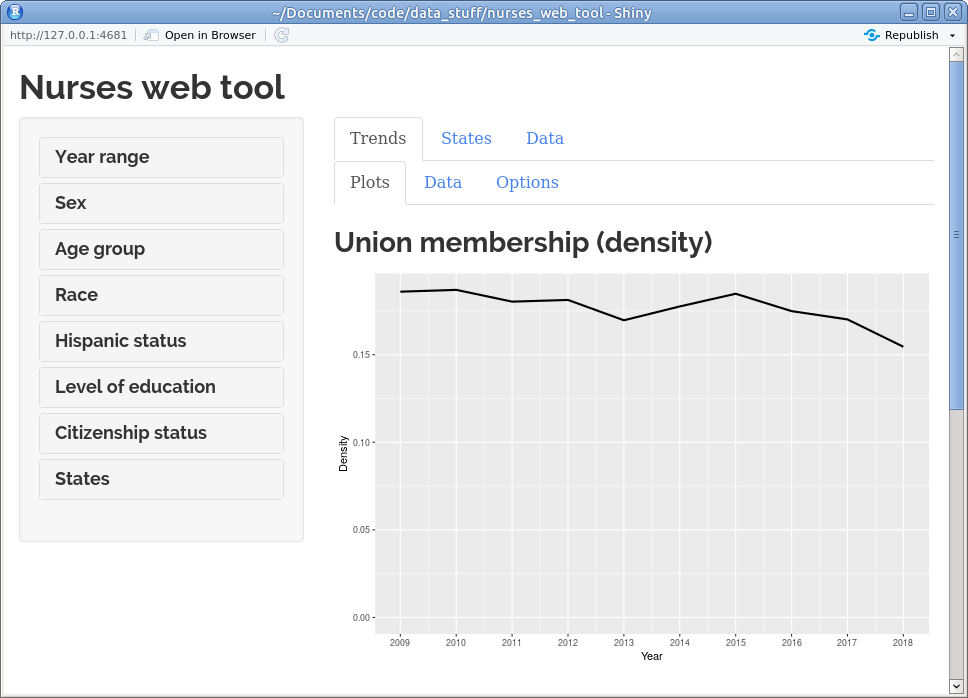
\includegraphics[width=0.7\textwidth]{images/opening_interface.png}
\end{center}
The various components of the interface are described in the next few
subsections.

\subsubsection{The filtering tools}

At the left side of the page you will notice a collection of drop down
menus, each of which corresponds to a variable in the data used by the
tool (which is described above). These are the \textit{filtering
 tools}. The web tool operates on the subset of the underlying data
selected using the filtering tools.

Clicking on a drop down menu in the filtering tools will reveal the
levels of that variable currently included in the subset of the data
being used by the web tool, displayed using checkboxes, slidebars, or
other selection widgets. For example, in the case of checkboxes, a
checked box indicates that the corresponding level of the variable is
currently included; an unchecked box indicates that it is not
included.

\subsubsection{The Trends tab}

Selecting the Trends tab at the top of the screen brings you to an
interface for exploring trends in union membership and union contract
coverage. This interface is described in detail below.

\subsubsection{The States tab}

Selecting the States tab at the top of the screen brings you to an
interface for creating chloropleth maps for displaying union
membership and union contract coverage per state. This interface is
described in detail below.

\subsubsection{The Data tab}

Selecting the Data tab allows you to view and download the data
selection currently being used by the tool. As described above, you
can modify the data selection using the filtering tools at the left
side of the page. The features of this tab are described in detail
below.

\subsection{Working with trends}

If you select the Trends tab, you will be presented with the following
interface:
\begin{center}
  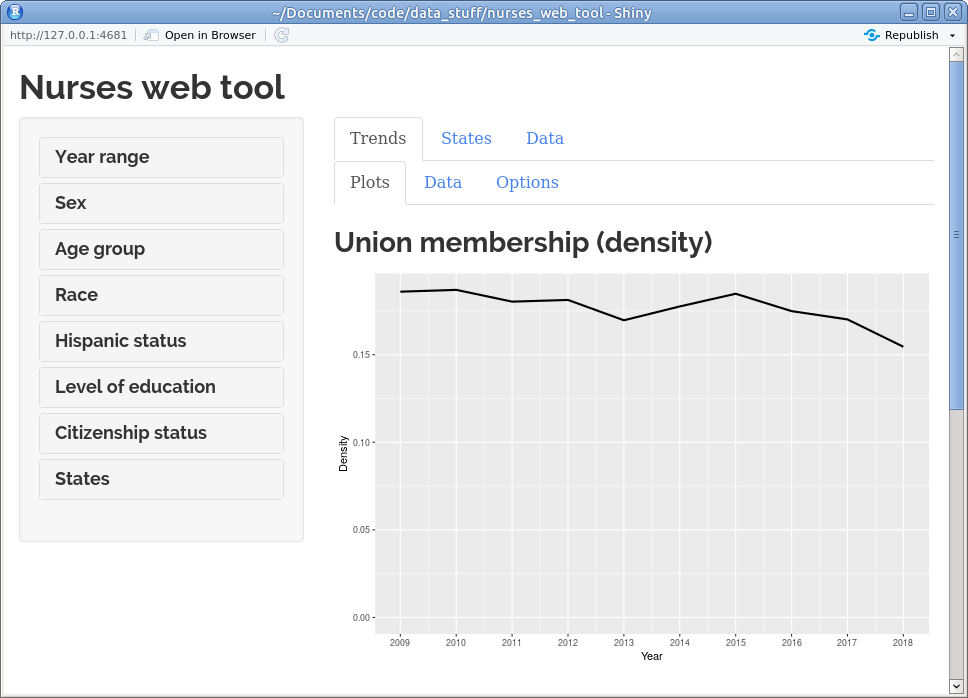
\includegraphics[width=0.7\textwidth]{images/trends_interface.png}
\end{center}
This interface allows you to explore trends in union membership and
union contract coverage. There are three sub-tabs: Plots, for viewing
the trend plots; Data, for viewing the data used to construct the
trend plots; and Options, for setting options related to the trend
plots.

To illustrate typical usage, we will work through several examples.
\begin{enumerate}
\item As a first example, let us create some basic trend plots showing
  union membership and union contract coverage trends for black,
  female nurses in the west coast states (California, Oregon, and
  Washington).

  First, select Trends \textrightarrow{} Plots to access the interface
  for viewing trend plots.

  Next we need to select the subset of data we want to work with. In
  this case, we want to examine black, female nurses in California,
  Oregon, and Washington. We can accomplish this using the filtering
  tools at the left side of the page. Click on the drop down menu
  labeled Sex in the filtering tools. You should see something like
  the following:
  \begin{center}
    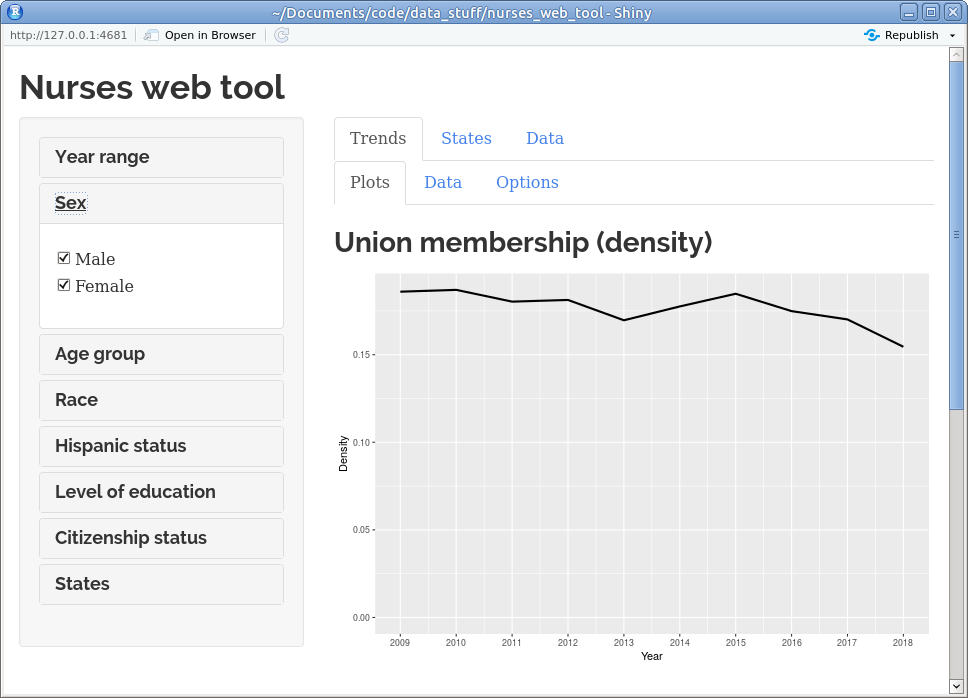
\includegraphics[width=0.7\textwidth]{images/trends_ex1/sex_selection.png}
  \end{center}
  We only want to examine female nurses, so uncheck the checkbox
  labeled Male. Restricting our attention to black nurses is similar:
  select the Race tab from the filtering tools and uncheck every
  checkbox except for the one labeled Black.

  Selecting our states of interest is a little different. Select the
  States tab from the filtering tools. You should see something like
  the following:
  \begin{center}
    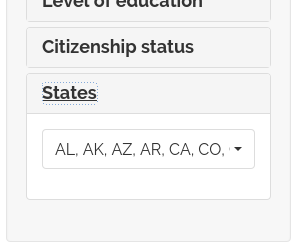
\includegraphics[width=0.3\textwidth]{images/trends_ex1/state_selection.png}
  \end{center}
  Clicking on the drop down menu allows you to select your states of
  choice:
  \begin{center}
    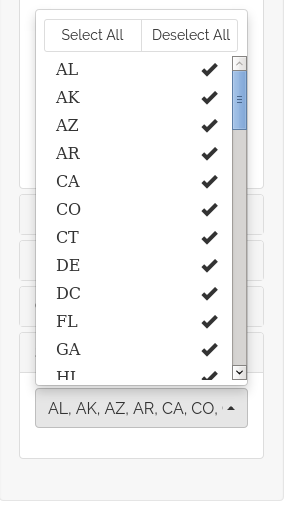
\includegraphics[width=0.3\textwidth]{images/trends_ex1/state_drop_down.png}
  \end{center}
  In this case, we want to select California, Oregon, and Washington
  (labeled CA, OR, and WA, respectively, in the drop down menu
  above). The easiest way to do this is to click Deselect All to
  remove all states from the selection, and then to select CA, OR, and
  WA from the drop down menu. Do this now.

  Note that you can hide a tab in the filtering tools by clicking on
  the tab again (just as you did to open the tab). Doing this, we end
  up with the following:
  \begin{center}
    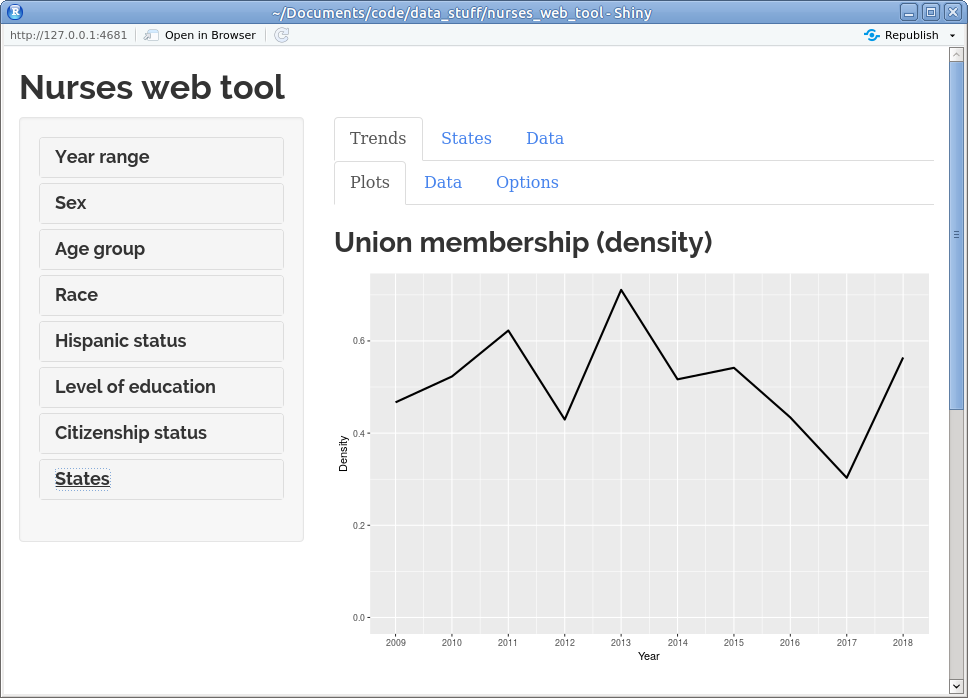
\includegraphics[width=0.7\textwidth]{images/trends_ex1/final_interface.png}
  \end{center}
  We now have two trend plots: one showing union membership over time,
  and one showing union contract coverage over time:
  \begin{center}
    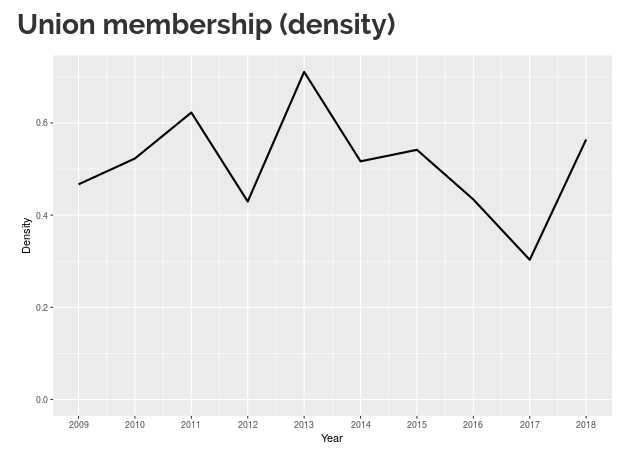
\includegraphics[width=0.49\linewidth]{images/trends_ex1/membership_trend.png}
    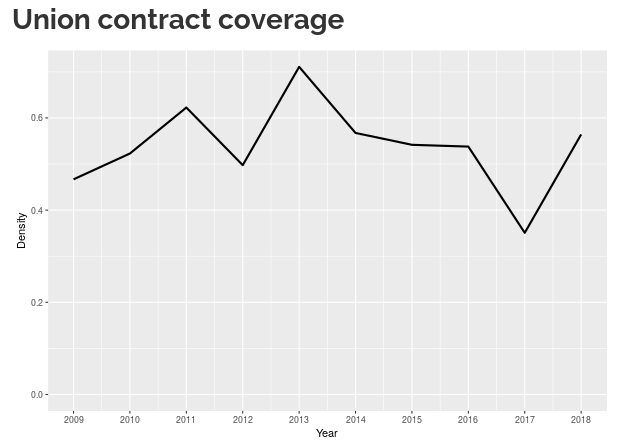
\includegraphics[width=0.49\linewidth]{images/trends_ex1/coverage_trend.png}
  \end{center}
  You can save either of these plots by right-clicking it and
  selecting the copy option from the drop-down menu, as you would with
  any other image on a webpage.

  Note that you can view the data used to generate the two trend plots
  by selecting Trends \textrightarrow{} Data. Doing this, you should
  see the following interface, which allows you to examine the data
  and download it in CSV format if you decide to perform custom
  analysis:
  \begin{center}
    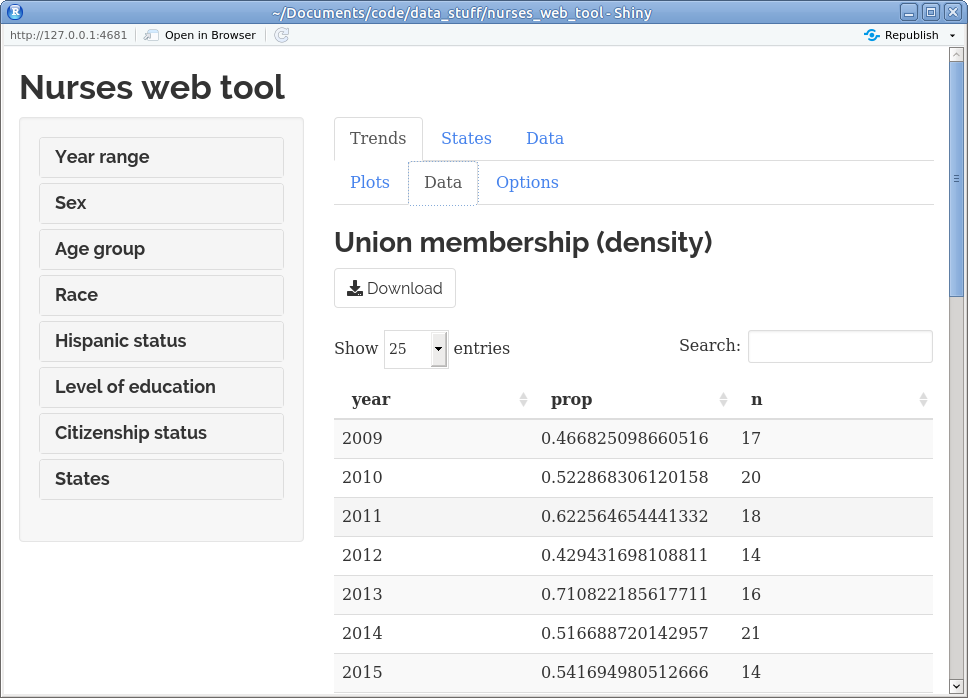
\includegraphics[width=0.7\textwidth]{images/trends_ex1/data_interface.png}
  \end{center}

\item For our second example, we will create trend plots showing the
  difference in union membership and the difference in union contract
  coverage among nurses in the age group 25-54 and nurses in the age
  group 55 and over.

  As in the previous example, go to Trends \textrightarrow{} Plots if
  you have not already.

  Next we want to select the subset of data we want to work with. In
  this case, we want to restrict our attention to nurses in the age
  group 25-54 and those in the age group 55 and over. To do this,
  select the Age group tab in the filtering tools at the left of the
  page. Make sure the right age groups are selected. Specifically, the
  selection should look as follows:
  \begin{center}
    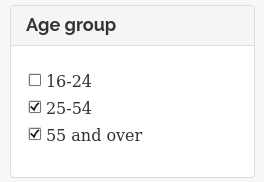
\includegraphics[width=0.3\textwidth]{images/trends_ex2/age_selection.png}
  \end{center}
  Right now our two trend plots display union membership and union
  contract coverage for nurses aged 25-54 and nurses aged 55 and over
  \emph{combined}. We want our plots to display the \emph{difference}
  between these two age groups. To do this, go to Trends
  \textrightarrow{} Options. You should see the following interface:
  \begin{center}
    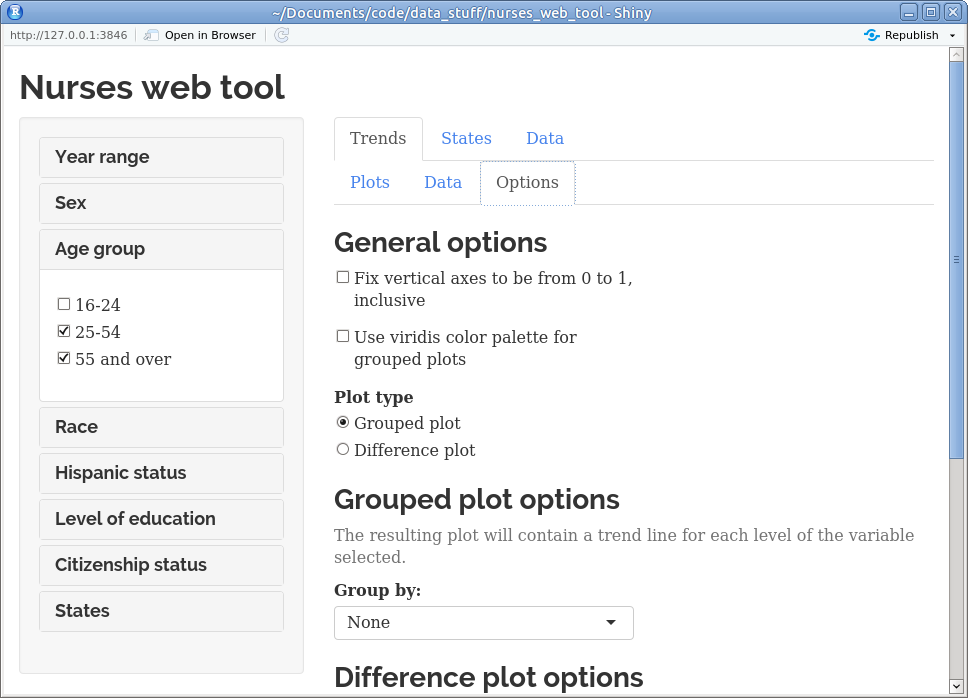
\includegraphics[width=0.7\textwidth]{images/trends_ex2/options_interface.png}
  \end{center}
  We want to take a look at the options for creating difference plots:
  \begin{center}
    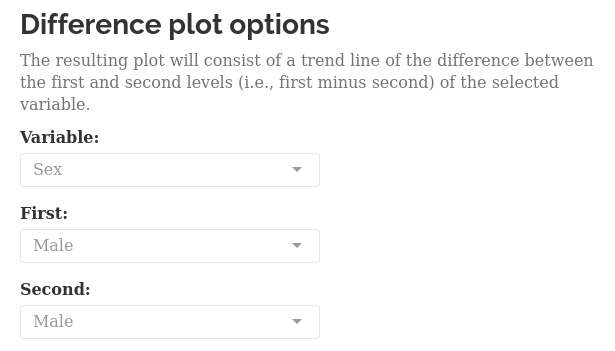
\includegraphics[width=0.7\textwidth]{images/trends_ex2/options_diff_plots.png}
  \end{center}
  These options may be currently disabled. Under the General options
  section, make sure the plot type is set to Difference plot:
  \begin{center}
    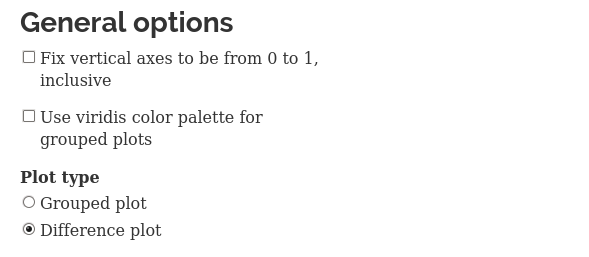
\includegraphics[width=0.7\textwidth]{images/trends_ex2/options_plot_type.png}
  \end{center}
  Next, go back to the difference plot options. Under the drop down
  menu labeled Variable, select Age group, and under the drop down
  menus labeled First and Second, select 25-54 and 55 and over,
  respectively. The options should now look like the following:
  \begin{center}
    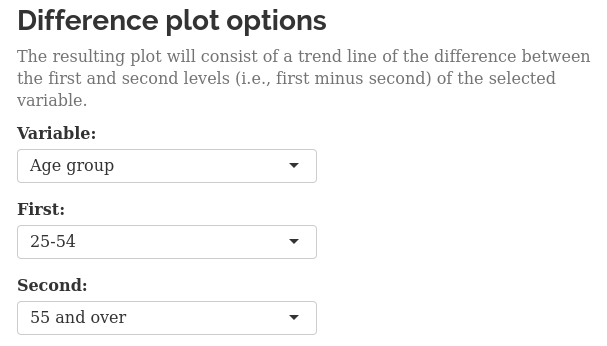
\includegraphics[width=0.7\textwidth]{images/trends_ex2/options_diff_plots2.png}
  \end{center}
  Now go back to Trends \textrightarrow{} Plots. We get the following
  two trend plots displaying the \emph{difference} in union membership
  and union contract coverage, respectively, between nurses aged 25-54
  and those aged 55 and over:
  \begin{center}
    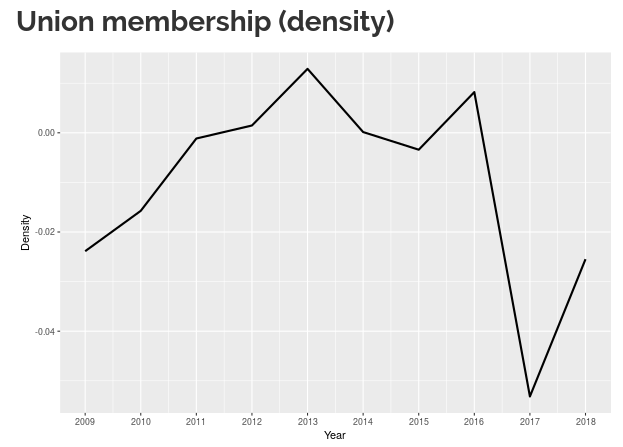
\includegraphics[width=0.49\linewidth]{images/trends_ex2/membership_trend.png}
    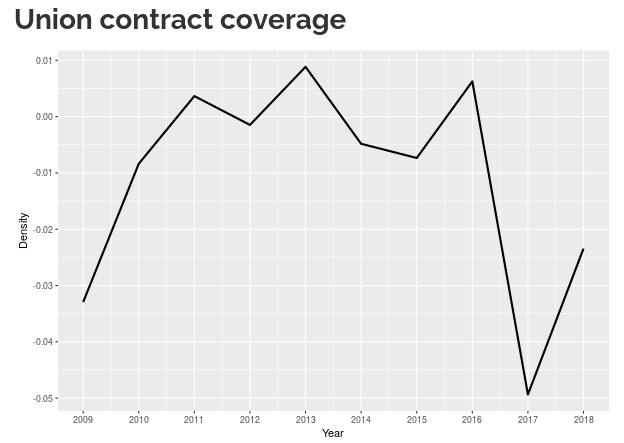
\includegraphics[width=0.49\linewidth]{images/trends_ex2/coverage_trend.png}
  \end{center}
  As in the previous example, you can view and download the data used
  to generate these plots under Trends \textrightarrow{} Data:
  \begin{center}
    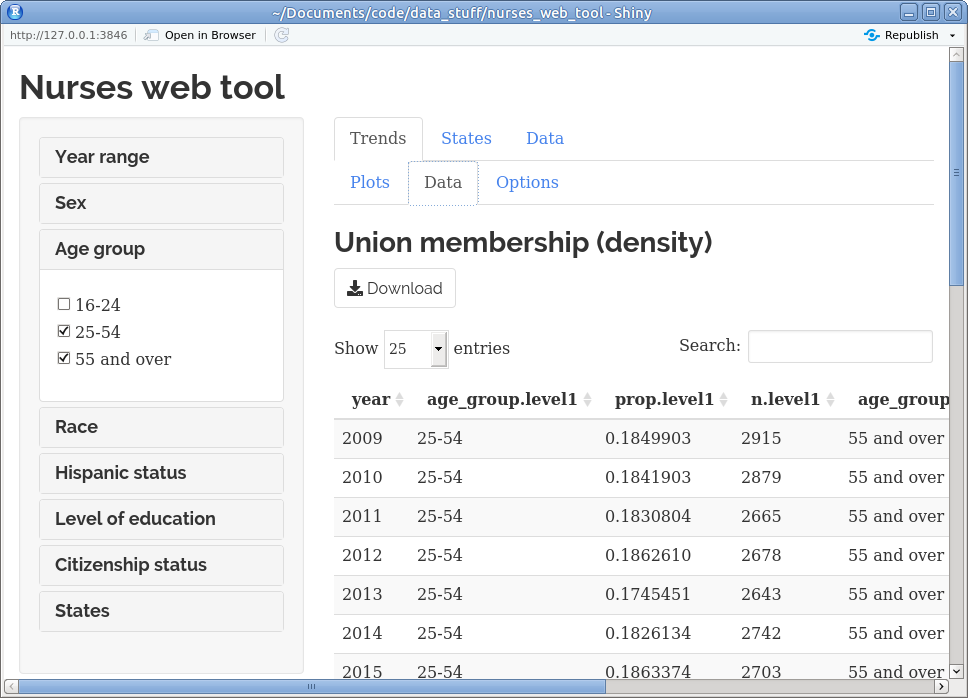
\includegraphics[width=0.7\textwidth]{images/trends_ex2/data_interface.png}
  \end{center}

\item In our third and final example we will create trend plots
  comparing both union membership and union contract coverage among
  nurses in the tri-state area (New York, New Jersey, and
  Pennsylvania) who are US native, foreign-born citizens, and
  foreign-born non-citizens.

  % TODO

\end{enumerate}

\subsection{Working with maps}

If you select the States tab, you will be presented with the following
interface:

\begin{center}
  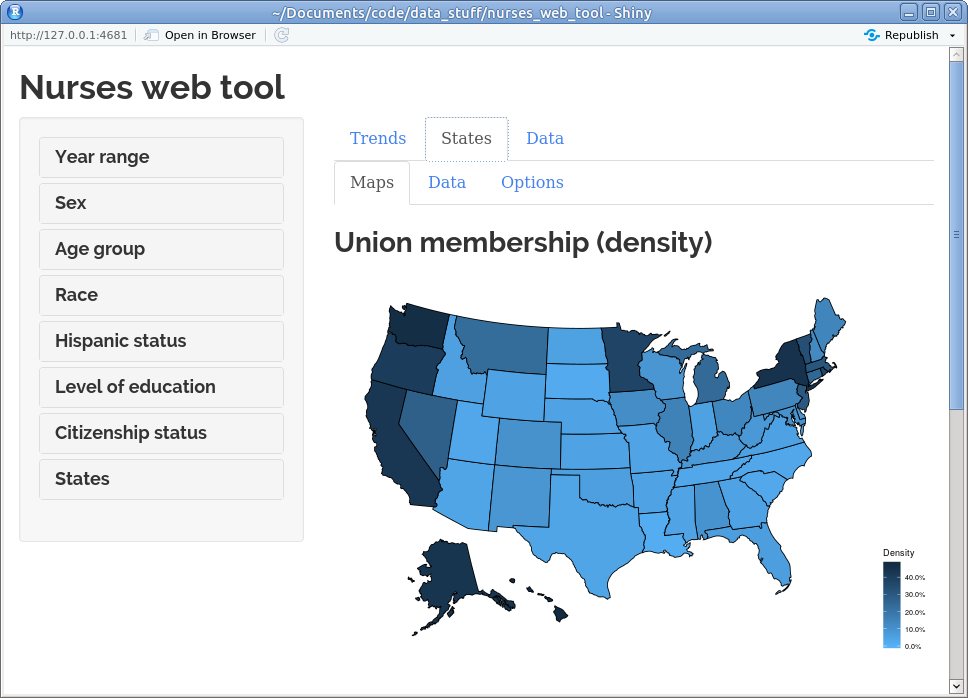
\includegraphics[width=0.7\textwidth]{images/states_interface.png}
\end{center}

This interface allows you to create chloropleth maps displaying union
membership and union contract coverage per state over the years
selected. There are three sub-tabs: Maps, for viewing the chloropleth
maps; Data, for viewing the data used to construct the chloropleth
maps; and Options, for setting options related to the chloropleth
maps.

To illustrate typical usage, we will work through several examples.
\begin{enumerate}
\item As a first example, we will create a chloropleth map showing
  union membership and union contract coverage among Hispanic nurses
  in the west coast states (California, Oregon, and Washington), over
  the years 2010 to 2015.

\item For our second example, we will create a chloropleth map showing
  union membership and contract coverage among all nurses in all
  states in the year 2011.

\end{enumerate}

\subsection{Examining the data selection}

If you select the Data tab, you will be presented with the following
interface:

\begin{center}
  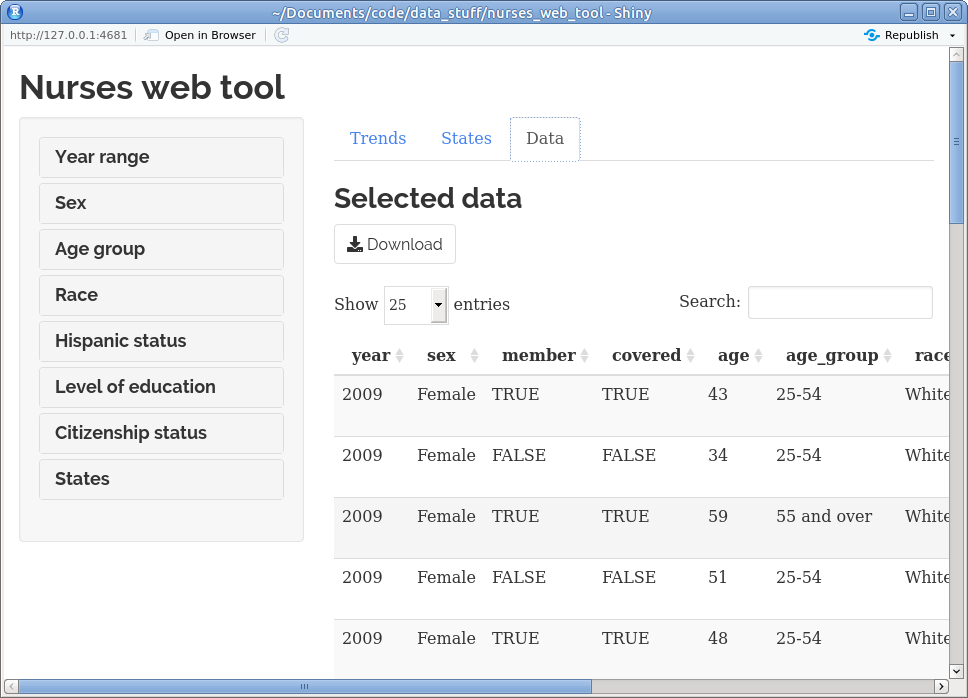
\includegraphics[width=0.7\textwidth]{images/data_interface.png}
\end{center}

% TODO

\end{document}
